% !TeX spellcheck = da_DK
% Setup document class.
%  This will always be the beamer class, but depending on the use of notes,
%  it can be annotated with the option [notes] or  [notes=only], depending
%  on whether notes should be included, or should be the only thing in
%  the document.

\documentclass[xcolor=table]{beamer}

%%%% USE WHEN PRINING HANDOUTS %%%%%

%\documentclass[xcolor=table, handout]{beamer}
%\usepackage{pgfpages}
%\pgfpagesuselayout{2 on 1}[a4paper,border shrink=5mm]

%%%%%%%


% Setup theme.
%\usetheme[
%%% options passed to the outer theme
%    progressstyle=fixedCircCnt,   %either fixedCircCnt, movCircCnt, or corner
%    rotationcw,          % change the rotation direction from counter-clockwise to clockwise
%    shownavsym          % show the navigation symbols
]{AAUsimple}

\usetheme[
%%% options passed to the outer theme
%    hidetitle,           % hide the (short) title in the sidebar
%    hideauthor,          % hide the (short) author in the sidebar
%    hideinstitute,       % hide the (short) institute in the bottom of the sidebar
%    shownavsym,          % show the navigation symbols
%    width=2cm,           % width of the sidebar (default is 2 cm)
    hideothersubsections,% hide all subsections but the subsections in the current section
%    hideallsubsections,  % hide all subsections
    left               % right of left position of sidebar (default is right)
%%% options passed to the color theme
%    lightheaderbg,       % use a light header background
  ]{AAUsidebar}

\setbeamercolor{alerted text}{fg=blue,bg=}


% Import preamble
%%% Initial things %%%
% Increase number of dimen registers
\usepackage{etex}
% Fix various issues with LaTeX2e
\usepackage{fixltx2e}
% Font package
\usepackage{fourier}


%%% Translations and character encodings %%%
% Enable use of several characters, including æ, ø and å
\usepackage[utf8]{inputenc}
% Danish language
\usepackage[danish]{babel}
% Use PostScript fonts instead of bitmap ones. Also does other stuff.
\usepackage[T1]{fontenc}
% Various LaTeX symbols
\usepackage{latexsym}
% Wider selection of colours
\usepackage{xcolor}
% Improved element justification
\usepackage{ragged2e}
% Font improvements
\usepackage{fix-cm}
% Enables various forms of lines, like double-underlining (\uuline{})
\usepackage{ulem}
% Sets the tolerance for distance between words, determining when to hyphenate.
\pretolerance=2500

\usepackage{rotating}

%%% Figures and tables (Floats) %%%
% Enable multi-rows and -columns
\usepackage{multirow}
\usepackage{multicol}
% Double, horizontal lines
\usepackage{hhline}
% Enables coloured tables
\usepackage{colortbl}
% Prettier tables
\usepackage{booktabs}


%%% Mathematic formulas %%%
% AMS math
\usepackage{amsmath}
\usepackage{amssymb}
% Extra fonts (for math, I think)
\usepackage{stmaryrd}
% Access text symbols
\usepackage{textcomp}
% Extend AMS
\usepackage{mathtools}
\usepackage{cancel}


%%% Graphics %%%
% Various image-commands
\usepackage{eso-pic}
% Use JPEG and PNG images
\usepackage{graphicx}

%%% Code listing %%%
\usepackage{color}
\definecolor{bluekeywords}{rgb}{0.13,0.13,1}
\definecolor{greencomments}{rgb}{0,0.5,0}
\definecolor{redstrings}{rgb}{0.9,0,0}

\usepackage{courier}

\usepackage{listings}

\lstset{language=[Sharp]C,
  captionpos=b,
  columns=fixed,
  numbers=left,
  numberstyle=\tiny,
  showspaces=false,
  showtabs=false,
  tabsize=3,
  breaklines=true,
  inputencoding=utf8,
  showstringspaces=false,
  breakatwhitespace=true,
  escapeinside={(*@}{@*)},
  commentstyle=\color{greencomments},
  keywordstyle=\color{bluekeywords},
  stringstyle=\color{redstrings},
  basicstyle=\ttfamily\small,
}

\lstdefinestyle{make}{tabsize=2}


%%% References, bibtex and URLs %%%
% Post URLs. Allows breaking at hyphens to help avoid long links.
\usepackage{url}
% Better cross references
\usepackage[danish]{varioref}
% Define a new 'leo' style for URL package, that will use a smaller font
\makeatletter
\def\url@leostyle{%
  \@ifundefined{selectfont}{\def\UrlFont{\sf}}{\def\UrlFont{\small\ttfamily}}
}
\makeatother
% And of course, use this new style
\urlstyle{leo}

\hypersetup{pdfstartview={Fit}}
%%%%%%%%%%%%%%%%%%%%%%%%%%%%%%%%%%%%%%%%%%%%%%%%
%Flowchart
\usepackage{tikz}
\usetikzlibrary{shapes.geometric, arrows, positioning, matrix, automata, positioning}
%%%%%%%%%%%%%%%%%%%%%%%%%%%%%%%%%%%%%%%%%%%%%%%%



\usepackage{color}
\definecolor{bluekeywords}{rgb}{0.13,0.13,1}
\definecolor{greencomments}{rgb}{0,0.5,0}
\definecolor{redstrings}{rgb}{0.9,0,0}
\usepackage{courier}
\usepackage{listings}

\lstset{ 
    literate={ø}{{\o}}1
         {æ}{{\ae}}1
         {å}{{\aa}}1
         {Ø}{{\O}}1
         {Æ}{{\AE}}1
         {Å}{{\AA}}1
         {§}{{\S}}1
}

%%% Colour definitions %%%
% Defines: gray
\definecolor{gray}{gray}{0.80}
% Defines: numbercolor
\definecolor{numbercolor}{gray}{0.7}
% Defines: shadecolor
\definecolor{shadecolor}{RGB}{33,26,82}
% Defines: aaublue

\definecolor{aaublue}{RGB}{33,26,82}


\colorlet{punct}{red!60!black}
\definecolor{background}{HTML}{EEEEEE}
\definecolor{delim}{RGB}{20,105,176}
\colorlet{numb}{magenta!60!black}

\newcommand*\rot{\rotatebox{90}}


\usepackage{pifont}
\newcommand{\cmark}{\ding{51}}%
\newcommand{\xmark}{\ding{55}}%

% Additional settings for boxes
\setbeamercolor{headerCol}{fg=black,bg=lightgray}
\setbeamercolor{bodyCol}{fg=white,bg=gray}
\setbeamercovered{transparent=20}

% Define document stuff
\title[TWAC]{Timely Wireless Arduino Communication}
\subtitle[Exam]{Exam}
\author[SW503E15]{SW503E15}
\date{January 22nd 2015}

\institute[
%  {\includegraphics[scale=0.2]{aau_segl}}\\ %insert a company, department or university logo
Software (SW5)\\
Aalborg University\\
Denmark
] % optional - is placed in the bottom of the sidebar on every slide
{% is placed on the title page
  Software (SW5)\\
  Aalborg University\\
  Denmark

  %there must be an empty line above this line - otherwise some unwanted space is added between the university and the country (I do not know why;( )
}

% Specify a logo on the titlepage (you can specify additional logos an include them in
% institute command below
\pgfdeclareimage[height=1.5cm]{titlepagelogo}{AAUgraphics/aau_logo_new} % placed on the title page
%\pgfdeclareimage[height=1.5cm]{titlepagelogo2}{graphics/aau_logo_new} % placed on the title page
\titlegraphic{% is placed on the bottom of the title page
  \pgfuseimage{titlepagelogo}
  %  \hspace{1cm}\pgfuseimage{titlepagelogo2}
}


\begin{document}

{\aauwavesbg
  \begin{frame}[plain,noframenumbering]
    \titlepage
  \end{frame}}

% ==================== SUBJECTS ======================
%\section{Udvikling af programmet}
	\begin{frame}{Udvikling af programmet}\framesubtitle{Indhold}
		 \begin{itemize}
		 	\item Arkitektur
		 	\item Funktionskomponenter
		 	\item Modellag
		 	\item Programmering
		 	\item Teknologier
		 	\item API
		 \end{itemize}
	\end{frame}
	\subsection{Arkitektur}
		\begin{frame}[t]{Arkitektur}\framesubtitle{MVC \& Komponenter}
			\begin{columns}[T]
				\begin{column}{.48\textwidth}
					\begin{itemize}
						\item Website
						\item Client--Server arkitektur
						\item MVC
						\begin{itemize}
							\item Model
							\item View
							\item Controller
						\end{itemize}
						\item Opdelt i funktionskomponenter
					\end{itemize}

				\end{column}
				\begin{column}{.48\textwidth}
					\begin{figure}
						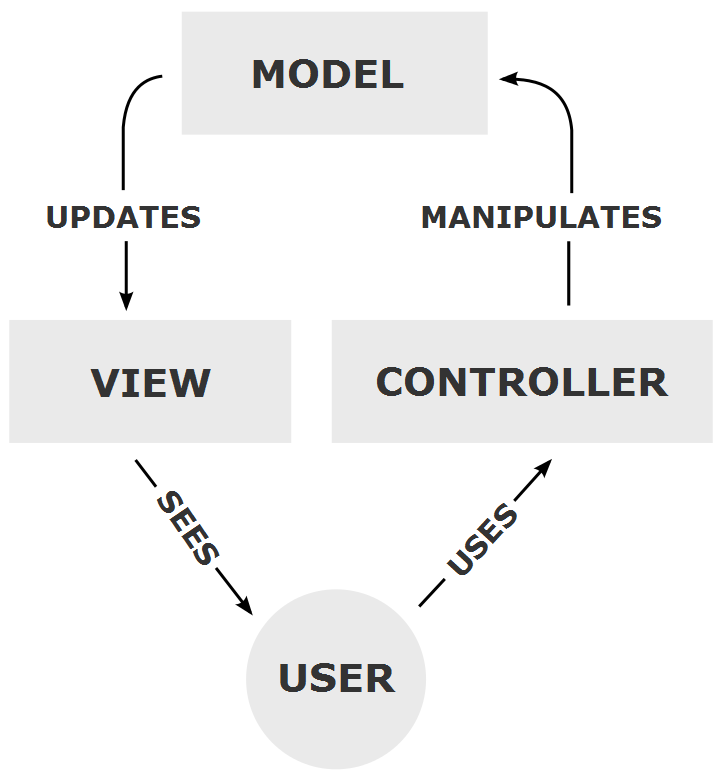
\includegraphics[width=1\textwidth]{images/MVC_2.png}
						\caption{MVC, figur af RegisFrey fra \url{wikipedia.org}}
					\end{figure}
				\end{column}
			\end{columns}
		\end{frame}
		
		\subsubsection{Funktionskomponenter}
		\begin{frame}[t]{Arkitektur}\framesubtitle{Funktionskomponenter}
			\begin{itemize}
				\item Funktionskomponenters adgange og afhængighedder
				\item Rækkefølge af komponenters implementering
			\end{itemize}
			%Topologisk sortering -> omvend reækkefølge -> implementer
			%Bruger > Tilbud > Indkøbsliste > Overvågning > Opskrift
			\vspace{-5pt}
			\begin{figure}[h!]
				\centering
				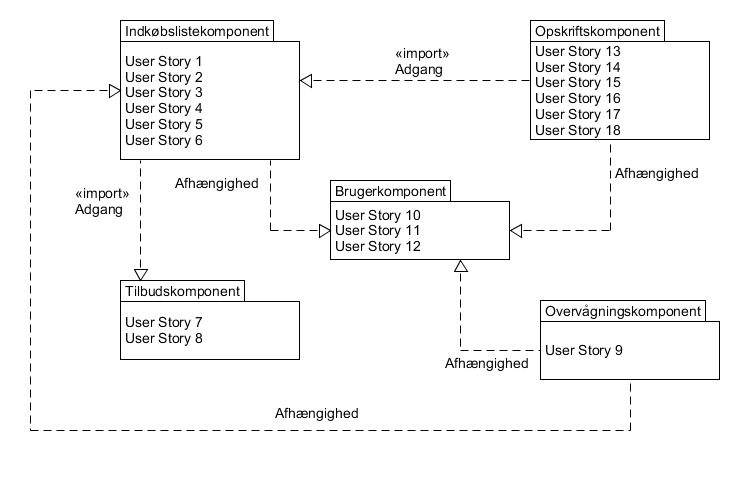
\includegraphics[width=1\textwidth]{images/Komponenter.png} % trim=1.4cm 6.1cm 6.5cm 1.8cm, clip, 
			\end{figure}
		\end{frame}

		\subsubsection{Modellag}
			\begin{frame}[t]{Arkitektur}\framesubtitle{Modellag}
				\begin{figure}
					
					\includegraphics<1-2>[trim=8.2cm 16.5cm 0.5cm 6.3cm, clip, width=1\textwidth]{images/PF_Model_UML_Simple.pdf} % ttrim=1.4cm 6.1cm 6.5cm 1.8cm, clip,
					\includegraphics<3>[width=0.5\textwidth]{images/UML_Pref_med_felter.png} % ttrim=1.4cm 6.1cm 6.5cm 1.8cm, clip,

				\end{figure}
				\begin{itemize}
					\item<2> Many-To-Many via bindeklasser med attributter
					\item<3> Problemer med modellaget
				\end{itemize}
			\end{frame}
		
		\subsection{Programmering}
			\begin{frame}{Programering}
				\begin{columns}
					\begin{column}{.48\textwidth}
						\begin{itemize}
							\item Git
							\begin{itemize}
								\item Branching
								\item Code-review
							\end{itemize}
							\item Pair Programming
							
						\end{itemize}

					\end{column}
					\begin{column}{.48\textwidth}
						\textbf{Branches:}
						\begin{itemize}
							\item master
							\item develop
							\item feature-xyz
							\item bugfix-abc
						\end{itemize}
					\end{column}
				\end{columns}
			\end{frame}


		\subsection{Teknologier}
			\begin{frame}[t]{Teknologier} %\framesubtitle{Udvikling intro}
				\begin{itemize}
					\item<1> ASP.NET
					\begin{itemize}
						\item<1> MVC
						\item<1> Razor view engine
						\item<1> Login system
					\end{itemize}
					\item<2> Entity Framework
					\begin{itemize}
						\item<2> Object--relational mapping
						\item<2> Code--first
						\item<2> Migrations
					\end{itemize}
					\item<3> Bootstrap
					\begin{itemize}
						\item<3> Responsiv layout
						\item<3> CSS--klasser og JS
					\end{itemize}
				\end{itemize}
			\end{frame}

		\subsection{eTilbudsavis API}
			\begin{frame}[t]{eTilbudsavis API}
			Kommunikation med API'en:
				\begin{enumerate}
					\item<1> POST api.etilbudsavis.dk/v2/\textbf{sessions}?api\_key=[...]
					\begin{itemize}
						\item<1> Modtag \texttt{token}
						\item<1> Beregn \texttt{signature} (SHA-256)
					\end{itemize}
					\item<2> GET api.etilbudsavis.dk/v2/\textbf{offers}?r\_lat=57\&r\_lng=9
					\begin{itemize}
						\item<2> Modtager 100 tilbud som JSON
						\item<2> Gentages til alle er modtaget (do..while)
						\item<2> Konverteres til \texttt{Offer}--klassen
					\end{itemize}
				\end{enumerate}
				\begin{itemize}
					\item<3> Er tidskrævende (60-300 sekunder)
					\item<3> Kan muligvis paralelliseres for bedre hastighed
					\item<3> Dataet kunne være bedre
				\end{itemize}
			\end{frame}
\section{Introduction}
\begin{frame}{Introduction}\framesubtitle{Overview}
    \begin{itemize}
        \item Initial Problem
        \item Problem Statement
        \item Development Process 
    \end{itemize}
\end{frame}
\subsection{``The Problem''}
\begin{frame}{Introduction}\framesubtitle{Initial Problem}
	\begin{itemize}
        \item Wired Communication vs. Wireless Communication
        \item Embedded System 
        \item Limited Resources
            \begin{itemize}
                \item Memmory
                \item Computational Power
                \item Radio Frequencies
            \end{itemize}
    \end{itemize}

\end{frame}
\begin{frame}{Introduction}\framesubtitle{Problem Statement}
\[
\left[
\begin{minipage}{\textwidth}
\centering
\begin{minipage}{0.96\textwidth}
How can a network of devices with radio transceivers of a single frequency communicate, such that any devices can send messages to other devices in the network, in a reliable while timely way?
\end{minipage}
\end{minipage}
\right]
\]
\end{frame}
\subsection{Development Process}
\begin{frame}{Introduction}\framesubtitle{Development Process}
    \begin{itemize}
        \item Scrum
        \item How should we itterate?
        \item Verify new ideas and design
        \item Test driven development?
        \begin{itemize}
            \item Dificult to test with hardware
            \item Design needs to be implemented for test
            \item Design flaws are caught late
        \end{itemize}
    \end{itemize}
\end{frame}


\section{Model-driven Development}
\begin{frame}[t]{Model-Driven Software Development (MDD)}

	\begin{columns}[T]
		\begin{column}{.48\textwidth}
			\centering
			Classic Software Development
			
			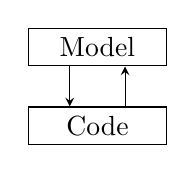
\begin{tikzpicture}[every node/.style={draw, minimum width = 50}, >=stealth]
				\node(model){Model};
				\node[below of=model](code){Code};
				\draw[->, transform canvas={xshift=-10}](model) -- (code);
				\draw[->, transform canvas={xshift= 10}](code) -- (model);
			\end{tikzpicture}
		\end{column}
		\begin{column}{.48\textwidth}
			\pause
			\centering	
			Model-driven Software Development
			
			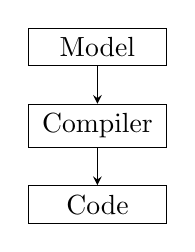
\begin{tikzpicture}[every node/.style={draw, minimum width = 50}, >=stealth]
				\node(model){Model};
				\node[below of=model](generator){Compiler};
				\node[below of=generator](code){Code};
				\draw[->](model) -- (generator);
				\draw[->](generator) -- (code);
			\end{tikzpicture}
		\end{column}
	\end{columns}
	
	\pause
	
	Advantages
	
	\begin{itemize}
		\item<+-> Better abstraction
		\item<+-> Models are easier to check for logical errors
		\item<+-> Models are easier to understand for non-programmers
	\end{itemize}
\end{frame}

\begin{frame}[t]{Model-Driven Software Development (MDD)}
	\framesubtitle{Our approch}
	
	{\centering
	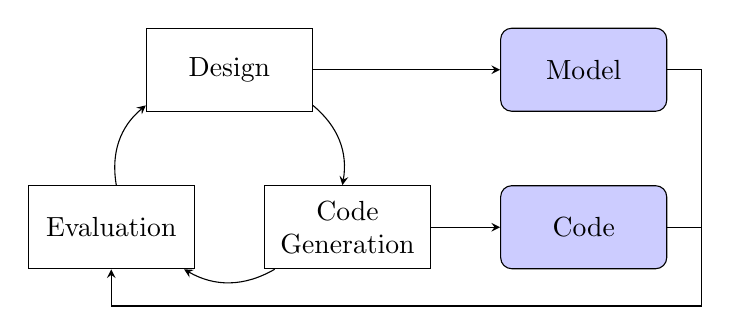
\begin{tikzpicture}[
			node distance = 75, 
			every node/.style={align=center, draw, minimum width=60, minimum height=30},
			>=stealth]
	
		\node(design) at (0,0) {Design};
		\node[rounded corners, fill = blue!20](model) at (4.5,0) {Model};
		\node(generation) at(1.5,-2){Code\\Generation};
		\node[rounded corners, fill = blue!20](code) at (4.5,-2){Code};
		\node(evaluation) at (-1.5,-2) {Evaluation};
	
		\draw[->] (design) -- (model);
		\draw[->] (generation) -- (code);
		
		\draw[->] (design) to[bend left] (generation);
		\draw[->] (generation) to[bend left] (evaluation);
		\draw[->] (evaluation) to[bend left] (design);
		
		\draw[->] (model) -| +(1.5,-3) -| (evaluation);
		\draw (code) -- +(1.5,0);
	\end{tikzpicture}
	}
	
	\smallskip
	
	\pause
	What is our reasoning?
	\begin{itemize}
		\item<+-> Models are easier to check for logical errors
		\item<+-> This also applies to model-model interaction
		\bigskip
		\item<+-> There exists tools to help with model checking
	\end{itemize}
\end{frame}

\section{Model checking}
\subsection{UPPAAL}
\begin{frame}[t]{Model checking}
	\framesubtitle{UPPAAL}
	
	\begin{block}{Description}
		\footnotesize 
		``Uppaal is an integrated tool environment for modeling, 
		validation and verification of real-time systems modeled as networks of timed automata, 
		extended with data types (bounded integers, arrays, etc.).''\footnote{http://www.uppaal.org/}
	\end{block}
	
	\begin{columns}[T]
		\begin{column}{.48\textwidth}
			\begin{itemize}
				\item Represented as automatas
				\item Querys can check for errors
			\end{itemize}
		\end{column}
		\begin{column}{.48\textwidth}
			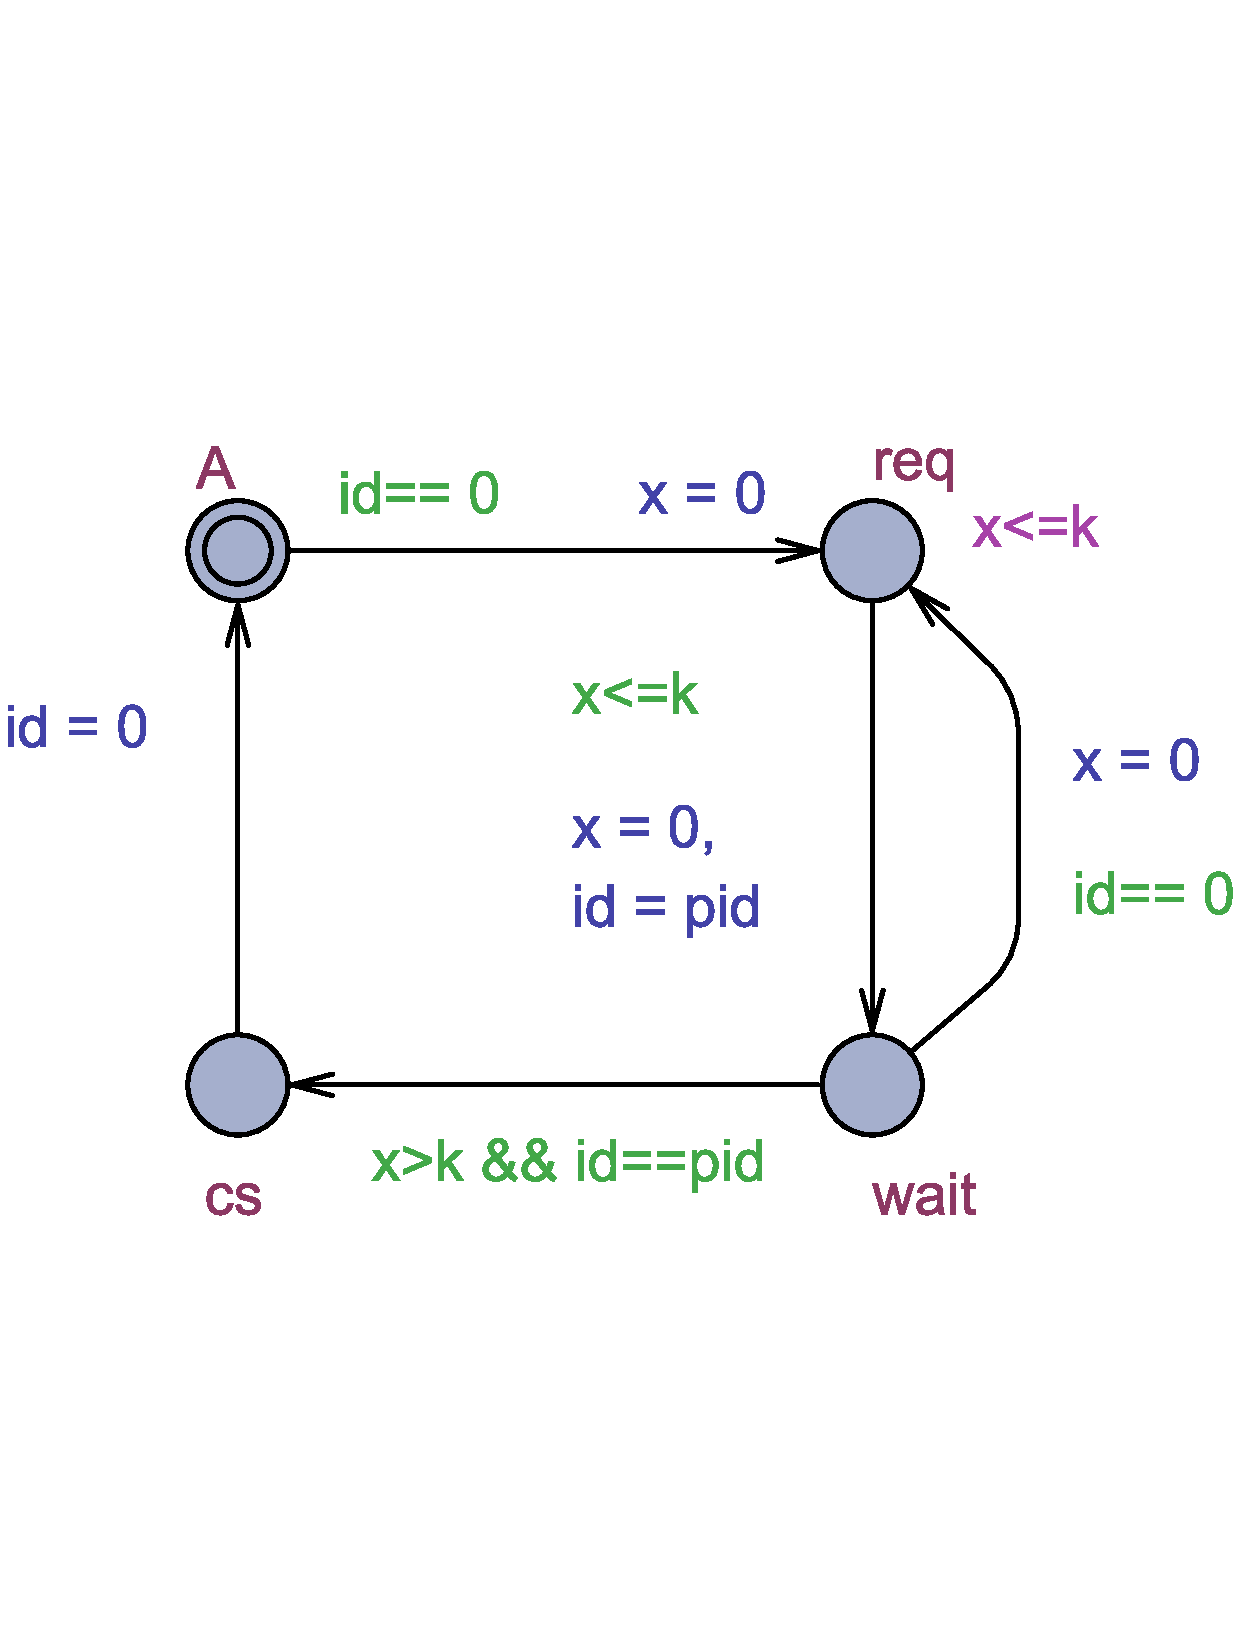
\includegraphics[trim=0 200 0 200,width=0.90\textwidth]{images/P.pdf}
		\end{column}
	\end{columns}
	\medskip
	\texttt{A[] forall (i:id\_t) forall (j:id\_t) P(i).cs \&\& P(j).cs imply i == j}
\end{frame}

\subsection{SMC}
\begin{frame}[t]{Model checking}
	\framesubtitle{Statistical Model Checking (SMC)}
	
	\begin{columns}[T]
		\begin{column}{.48\textwidth}
			Some great thing
			
			\begin{itemize}
				\item<+-> Some properties can not be guarenteed
				\item<+-> What are the chances of those being true?
			\end{itemize}
		\end{column}
		\begin{column}{.48\textwidth}
			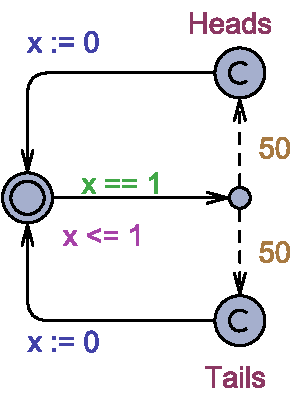
\includegraphics[trim=0 200 0 200,width=0.8\textwidth]{images/Simple_SMC.pdf}
		\end{column}
	\end{columns}
	
	\texttt{Pr[<=300000] (<> exists (i : id\_t) Coin(i).Tails)}
\end{frame}
\section{Problem Definition}
\subsection{Graph Problems}
\begin{frame}{The Problem Presented as Graphs}
\framesubtitle{How?}

\only<1,4>{
	\begin{itemize}
		\item Nodes are devices.
		\item Edges indicate which devices a device is in range of.
		
		\item<4> Weights indicate the chance of a transmission being received.
		
	\end{itemize}
}

\only<2>{
\begin{figure}
\centering
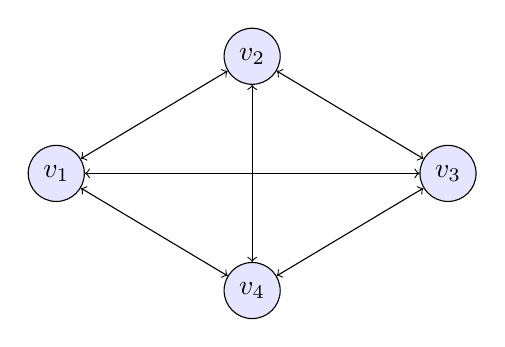
\begin{tikzpicture}  [
        node distance = 1 cm, 
        vertex/.style = {circle, draw, fill=blue!10}, 
        label/.style={fill=white},
        <->
    ]

    \node[draw=none](0){};
    \node[vertex, left  = 2cm of 0]   (1) {$v_1$};
    \node[vertex, above =     of 0]   (2) {$v_2$};
    \node[vertex, right = 2cm of 0]   (3) {$v_3$};
    \node[vertex, below =     of 0]   (4) {$v_4$};
    
    \draw (1) -- (2);
    \draw (1) -- (3);
    \draw (1) -- (4);
    \draw (2) -- (3);
    \draw (2) -- (4);
    \draw (3) -- (4);

\end{tikzpicture}
\end{figure}
Completely Connected Reliable Communication (CCRC).
}
\only<3>{
\begin{figure}
\centering
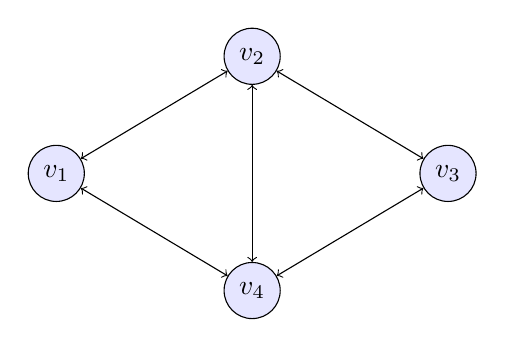
\begin{tikzpicture}  [
        node distance = 1 cm, 
        vertex/.style = {circle, draw, fill=blue!10}, 
        label/.style={fill=white},
        <->
    ]

    \node[draw=none](0){};
    \node[vertex, left  = 2cm of 0]   (1) {$v_1$};
    \node[vertex, above =     of 0]   (2) {$v_2$};
    \node[vertex, right = 2cm of 0]   (3) {$v_3$};
    \node[vertex, below =     of 0]   (4) {$v_4$};
    
    \draw (1) -- (2);
    \draw (1) -- (4);
    \draw (2) -- (3);
    \draw (2) -- (4);
    \draw (3) -- (4);

\end{tikzpicture}
\end{figure}
Strongly Connected Reliable Communication (SCRC).
}
\only<6>{
\begin{figure}
\centering
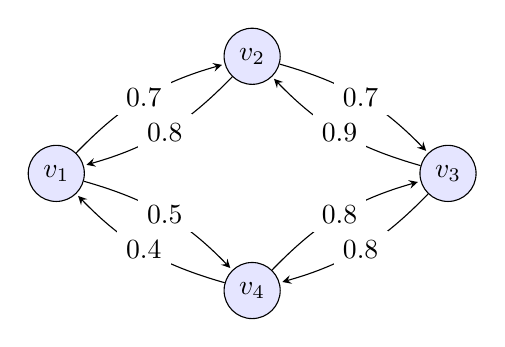
\begin{tikzpicture} [
        node distance = 1 cm, 
        vertex/.style = {circle, draw, fill=blue!10}, 
        edge/.style = {draw, -stealth, shorten >= 1pt},
        label/.style={fill=white}
    ]

    \node[draw=none](0){};
    \node[vertex, left =  2cm of 0]   (1) {$v_1$};
    \node[vertex, above=      of 0]   (2) {$v_2$};
    \node[vertex, right=  2cm of 0]   (3) {$v_3$};
    \node[vertex, below=      of 0]   (4) {$v_4$};
    
    \path[edge] (1) edge[bend left=15] node [label] {0.7} (2) edge[bend left=15] node [label] {0.5} (4);
    \path[edge] (2) edge[bend left=15] node [label] {0.8} (1) edge[bend left=15] node [label] {0.7} (3);
    \path[edge] (3) edge[bend left=15] node [label] {0.9} (2) edge[bend left=15] node [label] {0.8} (4);
    \path[edge] (4) edge[bend left=15] node [label] {0.4} (1) edge[bend left=15] node [label] {0.8} (3);
    
\end{tikzpicture}
\end{figure}
Strongly Connected Unreliable Communication (SCUC).
}

\only<5>{
\begin{figure}
\centering
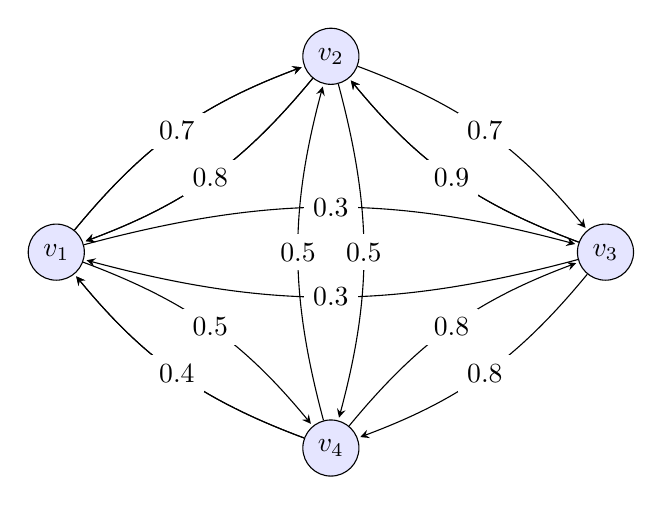
\begin{tikzpicture} [
        node distance = 1 cm, 
        vertex/.style = {circle, draw, fill=blue!10}, 
        edge/.style = {draw, -stealth, shorten >= 1pt},
        label/.style={fill=white}
    ]

    \node[draw=none](0){};
    \node[vertex, left =  3cm of 0]   (1) {$v_1$};
    \node[vertex, above=  2cm of 0]   (2) {$v_2$};
    \node[vertex, right=  3cm of 0]   (3) {$v_3$};
    \node[vertex, below=  2cm of 0]   (4) {$v_4$};
    
    \path[edge] (1) edge[bend left=15] node [label] {0.7} (2) edge[bend left=15] node [label] {0.5} (4);
    \path[edge] (1) edge[bend left=15] node [label] {0.7} (2) edge[bend left=15] node [label] {0.3} (3);
    \path[edge] (3) edge[bend left=15] node [label] {0.7} (2) edge[bend left=15] node [label] {0.3} (1);
    \path[edge] (2) edge[bend left=15] node [label] {0.7} (1) edge[bend left=15] node [label] {0.5} (4);
    \path[edge] (4) edge[bend left=15] node [label] {0.7} (1) edge[bend left=15] node [label] {0.5} (2);
    \path[edge] (2) edge[bend left=15] node [label] {0.8} (1) edge[bend left=15] node [label] {0.7} (3);
    \path[edge] (3) edge[bend left=15] node [label] {0.9} (2) edge[bend left=15] node [label] {0.8} (4);
    \path[edge] (4) edge[bend left=15] node [label] {0.4} (1) edge[bend left=15] node [label] {0.8} (3);
    
\end{tikzpicture}
\end{figure}
Completely Connected Unreliable Communication (CCUC).
}
\end{frame}

\begin{frame}{Time Division Multiple Access(TDMA)}
\subsection{TDMA Problem}
\framesubtitle{The generic method}
\begin{itemize}
	\item One frequency.
	\item Using the frequency in turns.
	\item Frame and time-slots.
\end{itemize}
\vspace{-15pt}
\begin{figure}
\centering
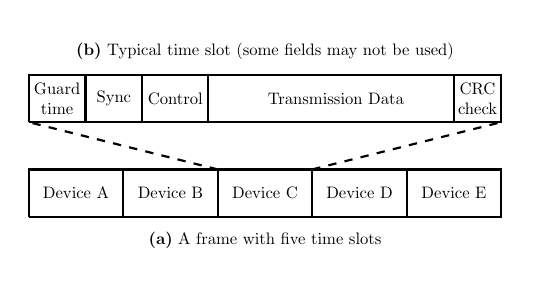
\begin{tikzpicture}[thick,scale=0.6, every node/.style={scale=0.6}]
    \path[draw] (-5,0) -- (-5,1) -- (5,1) -- (5,0) -- (-5,0)
                (-3,1) -- (-3,0)
                (-1,1) -- (-1,0)
                (1,1) -- (1,0)
                (3,1) -- (3,0);
                
    \node at (-4,0.5) {Device A};
    \node at (-2,0.5) {Device B};
    \node at (0,0.5) {Device C};
    \node at (2,0.5) {Device D};
    \node at (4,0.5) {Device E};
    
    \path[draw, dashed] (-1,1) -- (-5,2)
                        (1,1) -- (5,2);
    
    \path[draw] (-5,2) -- (-5,3) -- (5,3) -- (5,2) -- (-5,2)
                (-3.8,2) -- (-3.8,3)
                (-2.6,2) -- (-2.6,3)
                (-1.2,2) -- (-1.2,3)
                (4,2) -- (4,3);
    
    \node[text width=1cm, align=center] at (-4.4,2.5) {Guard\\time};
    \node at (-3.2,2.5) {Sync};
    \node at (-1.9,2.5) {Control};
    \node at (1.5,2.5) {Transmission Data};
    \node[text width=1cm, align=center] at (4.5,2.5) {CRC\\check};
    
    \path (-5,4) -- node{\textbf{(b)} Typical time slot (some fields may not be used)} (5,3);
    
    \path (5,-1) -- node{\textbf{(a)} A frame with five time slots} (-5,0);
\end{tikzpicture}
\end{figure}
\vspace{-15pt}
For our project:
	\begin{itemize}
		\item Devices should be able to join.
		\item The number of devices are not known in advance.
	\end{itemize}
\end{frame}

\section{CCRC}
\begin{frame}{Design of CCRC}
\framesubtitle{Changes from generic TDMA}

\begin{itemize}
	\item The TDMA solution for CCRC.
	\item Joining devices wait for Empty-Slot and then connects to the network.
\end{itemize}
\begin{figure}
\centering
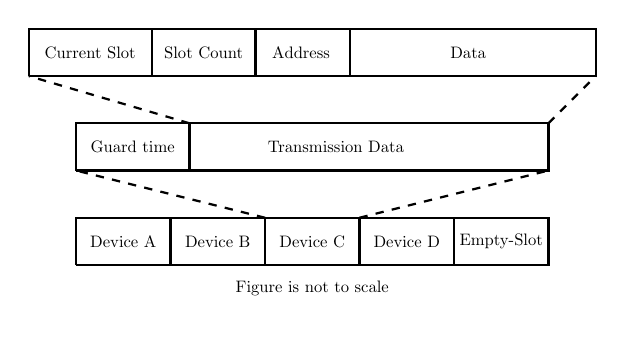
\begin{tikzpicture}[thick,scale=0.6, every node/.style={scale=0.6}]
    \path[draw] (-5,0) -- (-5,1) -- (5,1) -- (5,0) -- (-5,0)
                (-3,1) -- (-3,0)
                (-1,1) -- (-1,0)
                (1,1) -- (1,0)
                (3,1) -- (3,0);
                
    \node at (-4,0.5) {Device A};
    \node at (-2,0.5) {Device B};
    \node at (0,0.5) {Device C};
    \node at (2,0.5) {Device D};
    \node at (4,0.5) {Empty-Slot};
    
    \path[draw, dashed] (-1,1) -- (-5,2)
                        (1,1) -- (5,2);
    
    \path[draw] (-5,2) -- (-5,3) -- (5,3) -- (5,2) -- (-5,2)
                (-2.6,2) -- (-2.6,3);

    \node at (-3.8,2.5) {Guard time};
    \node at (0.5,2.5) {Transmission Data};

    \path[draw, dashed] (-2.6,3) -- (-6,4)
                        (5,3) -- (6,4);

    \path[draw] (-6,4) -- (-6,5) -- (6,5) -- (6,4) -- (-6,4)
    			(-3.4,4) -- (-3.4,5)
    			(-1.2,4) -- (-1.2,5)
    			(0.8,4) -- (0.8,5);

    \node at (-4.7,4.5) {Current Slot};
    \node at (-2.3,4.5) {Slot Count};
    \node[text width=1cm, align=center] at (-0.35,4.5) {Address};
    \node[text width=1cm, align=center] at (3.3,4.5) {Data};
    
    \path (5,-1) -- node{Figure is not to scale} (-5,0);

\end{tikzpicture}
\end{figure}
\begin{itemize}
\item Presentation of CCRC in UPPAAL.
\end{itemize}
\end{frame}

\section{Simultaneous connect}
\subsection{Multiple Startup}
\begin{frame}{Multiple Startup}
  \begin{itemize}
    \item CCUC assumptions
    \item Message redundancy
    \item Multiple connect
  \end{itemize}
\end{frame}

\subsection{Multiple Connect}
\begin{frame}{Multiple Connect}
  \begin{itemize}
    \item CCUC assumptions
    \item Message redundancy
    \item Multiple connect
  \end{itemize}
\end{frame}

\begin{frame}{Overview}
  \begin{itemize}
    \item CCUC assumptions
    \item Message redundancy
    \item Multiple connect
  \end{itemize}
\end{frame}
\subsection{CCUC assumptions}
\begin{frame}{CCUC assumptions}
The CCUC-problem describes a completely connected graph but in this scenario there is not a guarantee that the transmission will be received; all devices are still in the range of each other.
\end{frame}

\section{CCUC}
\subsection{CCUC Solution}

\begin{frame}{CCUC Improvements}
\framesubtitle{Message Redundancy}
\only<1>{
  \begin{itemize}
    \item Pros
      \begin{itemize}
    	\item Increases reliability
    	\item Simple to implement
  	  \end{itemize}
    \item Cons
      \begin{itemize}
    	\item Time consuming
    	\item Naïve solution
  	  \end{itemize}
  \end{itemize}
}
\only<2>{
\begin{figure}
\centering
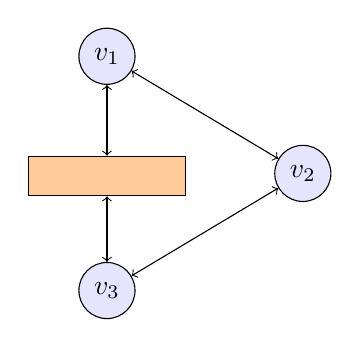
\begin{tikzpicture}  [
        node distance = 1 cm, 
        vertex/.style = {circle, draw, fill=blue!10}, 
        label/.style = {fill=white},
        block/.style = {rectangle, draw, fill=orange!40, minimum height = 5mm, minimum width = 20mm},
        <->
    ]

    \node[draw=none](0){};
    \node[vertex, above =     of 0]   (2) {$v_1$};
    \node[block,  below = 9mm of 2]   (1) {};
    \node[vertex, right = 2cm of 0]   (3) {$v_2$};
    \node[vertex, below =     of 0]   (4) {$v_3$};
    
    \draw (2) -- (3);
    \draw (3) -- (4);
    \draw (1) -- (2);
    \draw (1) -- (4);
%    \draw (2) -- (4);
%    \draw (3) -- (4);

\end{tikzpicture}
\end{figure}
Text here
}
\end{frame}

\section{Implementation}
    \subsection{Automated Code Generation}
    \begin{frame}[t]{Code Generation From Model}\framesubtitle{Model Driven Development}
        Ideally
        \begin{enumerate}
            \item Make model
            \item Verify it
            \item ??? (Automated Code Generation)
            \item Implementation is over
        \end{enumerate}
        \bigskip
        \begin{itemize}
            \item <2->Assuming the 3rd step is correct then it will work, because the model works!
            \item <3->However this is a \textcolor{orange}{difficult} problem, and code generation will be done manually 
        \end{itemize}
    \end{frame}
    \subsection{Implementing for the Arduino}
    \begin{frame}[t]{Implementing for the Arduino}\framesubtitle{Platform and toolchain}
        \begin{itemize}
            \item C/C++-like language
            \item $< 500$ LOC
            \item Uses a Library (RadioHead) to communicate
            \item Relatively simple to make given the model
            \item Hardest problem being synchronization related
            \item Uses 8560 bytes out of 32256 bytes of storage (26 \%)
            \item Uses 672 bytes of 2048 bytes of memory (32 \%)
        \end{itemize}

    \end{frame}
    \begin{frame}[t]{Implementing for the Arduino}\framesubtitle{Usercode}
        \begin{itemize}
            \item \texttt{void userCodeRunonce()}
            \begin{itemize}
                \item Once pr. time-slot
                \item WCET must be less than the time set to execute user code in
            \end{itemize}
            \item \texttt{void userCodeRepeat()}
            \begin{itemize}
                \item Used to fill the rest of the user code execution time
                \item WCET must be less than the guard time before transmitting
            \end{itemize}
            \item \texttt{void userSensorPoll()}
            \begin{itemize}
                \item Can be enabled to pool sensor while receiving
                \item WCET should be short i.e. sub-millisecond
            \end{itemize}
        \end{itemize}

    \end{frame}

\section{Demonstration}
    \subsection{Remote}
    \begin{frame}[t]{Demonstration}\framesubtitle{Remote controlled presentation.}
        \begin{itemize}
            \item 2 devices
            \item Reads from sensor
            \item Sends special byte
            \item Device connected to PC reads
            \item Bash script reads from device
            \item VBScript sends keystroke to PDF-reader
            \item Effect: Can control slides from remote!
            \item (WCET without packetloss: 600 ms * 3 = 1800 ms)
        \end{itemize}
    \end{frame}
    \subsection{Lightshow}
    \begin{frame}[t]{Demonstration}\framesubtitle{Lightshow!}
        \begin{itemize}
            \item 3 devices
            \item Usercode!
            \item Can start multiple at the same time
            \item Green LED on while sending
            \item Red LED on while receiving
            \item Multiple buttons turning on LEDs/actuators
            \item (Note: Timeslot is 2 x desired length for demonstrative purposes.)
        \end{itemize}
    \end{frame}

\section{Epilogue}
     \begin{frame}[t]{Epilogue}\framesubtitle{Schedule}
        \begin{itemize}
            \item Improvements on Current Work
            \item Conclusion
            \item Future Works
        \end{itemize}
    \end{frame}

    \subsection{Improvements on Current Work}
        \begin{frame}[t]{Epilogue}\framesubtitle{Developed Improvements}
            \begin{columns}[T]
                \begin{column}{0.48\textwidth}
                    \begin{itemize}
                        \item Simultaneous Connect
                        \item Frame Defragmentation
                            \begin{itemize}
                                \item Decremental Gradual Defragmentation
                                \item Jumping Defragmentation
                                \item Automatic Insertion
                            \end{itemize}
                    \end{itemize}
                \end{column}
                \begin{column}{.48\textwidth}
                    \begin{figure}
                        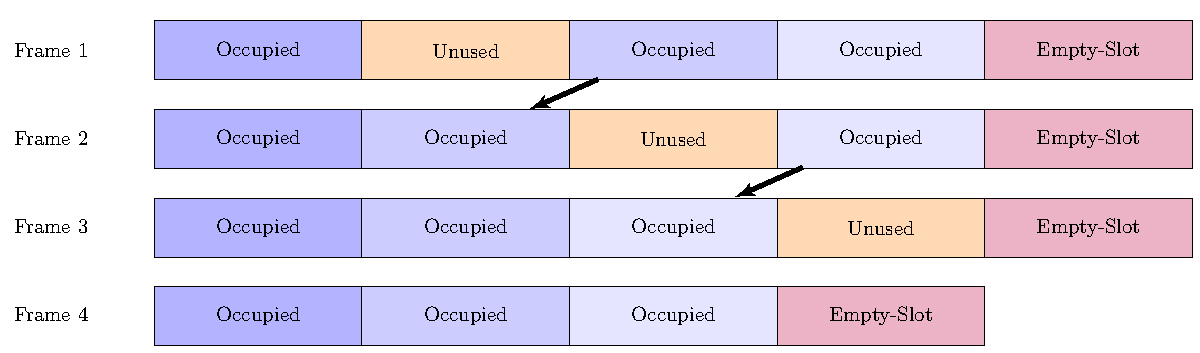
\includegraphics[width=1\textwidth]{images/dgd.pdf}
                    \end{figure}
                    \begin{figure}
                        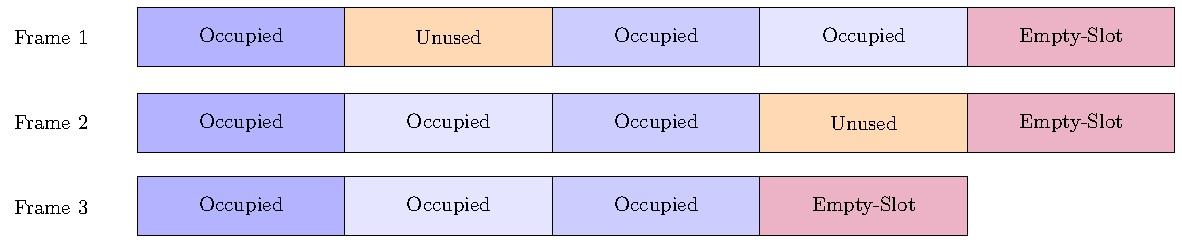
\includegraphics[width=1\textwidth]{images/jd.pdf}
                    \end{figure}
                    \begin{figure}
                        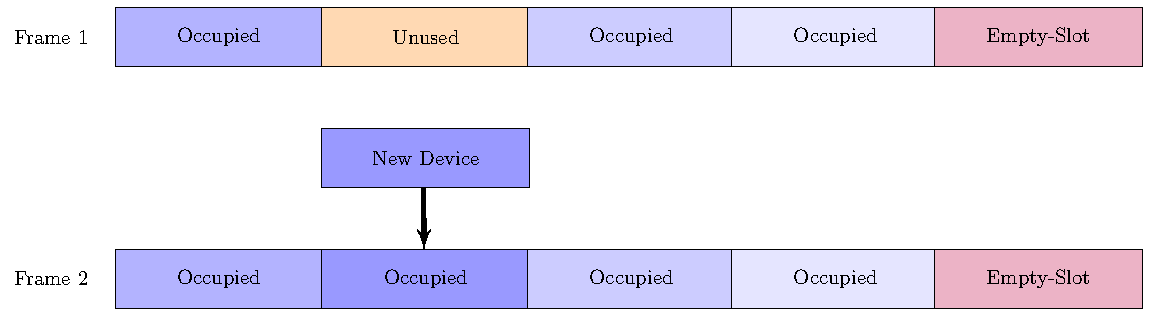
\includegraphics[width=1\textwidth]{images/aiut.pdf}
                    \end{figure}
                \end{column}
            \end{columns}
        \end{frame}

 %       \begin{frame}[t]{Epilogue}\framesubtitle{Further Points of Interest}    
 %           \begin{itemize}
 %               \item Interrupt Library
 %               \item Operating Speed
 %                   \begin{itemize}
 %                           \item Software Improvements
 %                           \item Hardware Improvements
 %                   \end{itemize}
 %           \end{itemize}
 %       \end{frame}

    \subsection{Conclusion}
        \begin{frame}[t]{Epilogue}\framesubtitle{Conclusion}
        \begin{columns}[T]
            \begin{column}{0.48\textwidth}
                \begin{itemize}
                    \item Development Method
                    \item Adaptability to Reality
                        \begin{itemize}
                            \item Uncertainty
                            \item Physical Complications
                        \end{itemize}
                    \item Requirements
                        \begin{itemize}
                            \item Death Detection
                            \item Echo  
                        \end{itemize}
                \end{itemize}
            \end{column}
            \begin{column}{.48\textwidth}

\begin{figure}
\centering
\resizebox{5.25cm}{!}{%
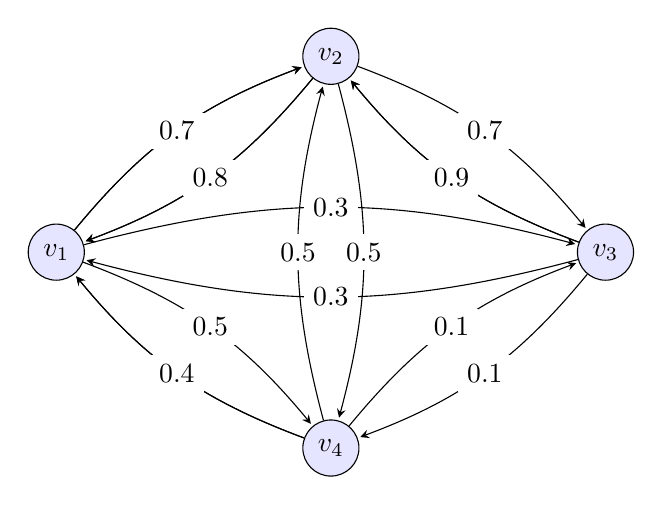
\begin{tikzpicture} [
        node distance = 1 cm,   
        vertex/.style = {circle, draw, fill=blue!10}, 
        edge/.style = {draw, -stealth, shorten >= 1pt},
        label/.style={fill=white}
    ]

    \node[draw=none](0){};
    \node[vertex, left =  3cm of 0]   (1) {$v_1$};
    \node[vertex, above=  2cm of 0]   (2) {$v_2$};
    \node[vertex, right=  3cm of 0]   (3) {$v_3$};
    \node[vertex, below=  2cm of 0]   (4) {$v_4$};
    
    \path[edge] (1) edge[bend left=15] node [label] {0.7} (2) edge[bend left=15] node [label] {0.5} (4);
    \path[edge] (1) edge[bend left=15] node [label] {0.7} (2) edge[bend left=15] node [label] {0.3} (3);
    \path[edge] (3) edge[bend left=15] node [label] {0.7} (2) edge[bend left=15] node [label] {0.3} (1);
    \path[edge] (2) edge[bend left=15] node [label] {0.7} (1) edge[bend left=15] node [label] {0.5} (4);
    \path[edge] (4) edge[bend left=15] node [label] {0.7} (1) edge[bend left=15] node [label] {0.5} (2);
    \path[edge] (2) edge[bend left=15] node [label] {0.8} (1) edge[bend left=15] node [label] {0.7} (3);
    \path[edge] (3) edge[bend left=15] node [label] {0.9} (2) edge[bend left=15] node [label] {0.1} (4);
    \path[edge] (4) edge[bend left=15] node [label] {0.4} (1) edge[bend left=15] node [label] {0.1} (3);
    
\end{tikzpicture}
}%
\end{figure}

            \end{column}
        \end{columns}
        \end{frame}

    \subsection{Future Works}
        \begin{frame}[t]{Epilogue}\framesubtitle{Strongly Connected}
            \begin{columns}[T]
                \begin{column}{0.48\textwidth}
                    \begin{itemize}
                        \item Strongly-Connected
                        %Provides many new problems in itself, timeslot, previous work must be reconsidered etc.
                        \item Error Reconfiguration
                        \item Device Authentication
                        \item Beyond the Protocol
                        %Specific use case tuning, Fire Alarm, Home Automisation etc.
                    \end{itemize}
                \end{column}
            \begin{column}{.48\textwidth}
                
                \begin{figure}
                \centering
                \resizebox{0.6cm}{!}{%
                    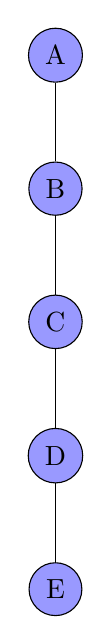
\begin{tikzpicture} [device/.style={circle, fill=blue!40, draw}]
\node[device](d1){A};
\node[device, below=of d1](d2){B};
\node[device, below=of d2](d3){C};
\node[device, below=of d3](d4){D};
\node[device, below=of d4](d5){E};

\draw (d1) -- (d2) -- (d3) -- (d4) -- (d5);
\end{tikzpicture}
}%
                \end{figure}
            \end{column}
        \end{columns}
        \end{frame}


% ====================================================

% Final slide
{\aauwavesbg
  \begin{frame}[plain,noframenumbering]
    \finalpage{\texttt{throw new PresentationIsOverException();}}
  \end{frame}}

\end{document}
